\begin{flushright} {\tiny {\color{gray} pair\_mini.tex}} \end{flushright}
%~~~~~~~~~~~~~~~~~~~~~~~~~~~~~~~~~~~~~~~~~~~~~~~~~~~~~~~~~~~~~~~~~~~~~~~~~~~~~~~~~~~~~~~~~~~~~~~~~~

\noindent
\begin{minipage}{0.48\textwidth}
The \index{general}{MINI element} MINI element was first introduced in Arnold \etal, 1984 \cite{arbf84}.
It is also discussed in Section~3.6.1 of \textcite{john16} (2016) and in Section~6.1 
of \textcite{bobf08} (2008).

As explained in Braess \cite{braess}, since the support of the bubble is restricted to the element, 
the associated variable (dofs living on the bubble) can be eliminated from the resulting 
system of linear equations by static condensation. \index{general}{Static Condensation}
Also, the MINI element is cheaper than the Taylor-Hood element but it is commonly accepted
that it yields a poorer approximation of the pressure.
\end{minipage}\hfill
\begin{minipage}{0.48\textwidth}
\begin{flushright} {\tiny {\color{gray} (tikz\_mini.tex)}} \end{flushright}
%~~~~~~~~~~~~~~~~~~~~~~~~~~~~~~~~~~~~~~~~~~~~~~~~~~~~~~~~~~~~~~~~~~~~~~~~~~~~~~~~~~~~~~~~~~~~~~~~~~

\begin{center}
\begin{tikzpicture}
%\draw[fill=gray!23,gray!23](0,0) rectangle (5,5);
%\draw[step=0.5cm,gray,very thin] (0,0) grid (5,3.5); %background grid
\draw[thick] (1,0.5) -- (4,1)  -- (3,3) -- cycle; %1-9-2-6-5

%pressure nodes
\draw[violet] (1,0.5) circle (4pt); % 0 
\draw[violet] (4,1) circle (4pt); % 1 
\draw[violet] (3,3) circle (4pt); % 2 

%velocity nodes
\draw[black,fill=teal] (1,0.5)   circle (2pt);
\draw[black,fill=teal] (4,1)   circle (2pt);
\draw[black,fill=teal] (3,3)   circle (2pt);
\draw[black,fill=teal] (2.75,1.5)   circle (2pt);

% legend
\draw[black,fill=teal] (3.1,0.2) circle (2pt); \node[] at (3.4,0.2) {$\vec\upnu$};
\draw[violet] (4.1,0.2) circle (4pt); 
\node[] at (4.4,0.2) {$p$};
\node[] at (2.5,3.75) {4 vel. nodes, 3 press. nodes};
\end{tikzpicture}\\
\end{center}


\end{minipage}

\begin{remark}
Note that Franca \& Oliveira (2003) \cite{frol03} propose an equal-order-linear-continuous 
velocity-pressure variables which is enriched 
with velocity {\it and} pressure bubble functions to model the Stokes problem. 
They show by static condensation that
these bubble functions give rise to a stabilized method involving least-squares forms of 
the momentum and of the
continuity equations. In some cases their approach recovers 
the MINI element. Also check Ganesan \etal (2008) \cite{gamt08}.
\end{remark}


The 3D MINI element is not very common but it is used for instance in Pichelin \& Coupez (1998) 
\cite{pico98}. It is also said to be LBB stable in Reddy \cite[p180]{reddybook2}.

\begin{center}
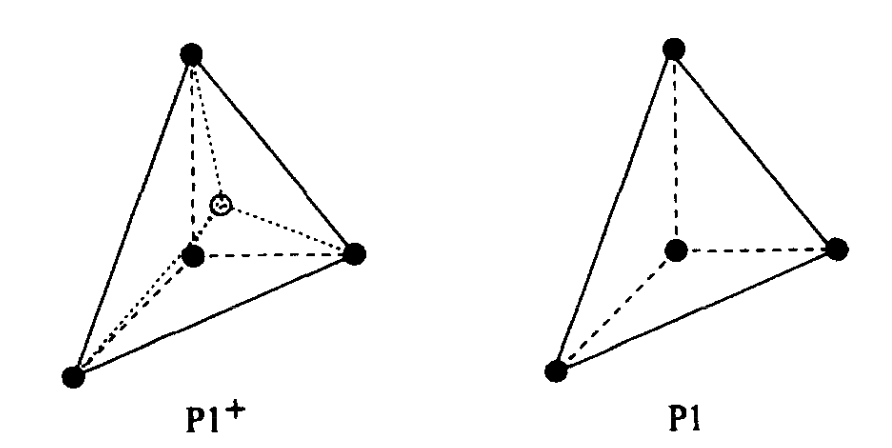
\includegraphics[width=8cm]{images/mini/mini3D}\\
{\captionfont Velocity and pressure nodes for the 3D MINI element, taken from \cite{pico98}}
\end{center}

Note that this element is used in Braess \& Wriggers (2000) \cite{brwr00} 
in the context of Arbitrary Lagrangian Eulerian 
finite element analysis of free surface flows, and also 
in Zlotnik \etal (2007) \cite{zldf07} for subduction with X-FEM technique. 
\index{general}{X-FEM}.

This element is implemented in \stone~120.
